\section{Результаты тестирования}

\subsection{ROS}
\begin{frame}{ROS - влияние различных факторов}
	Размера буфера:
	\begin{columns}[onlytextwidth]
		\begin{column}{0.45\textwidth}
			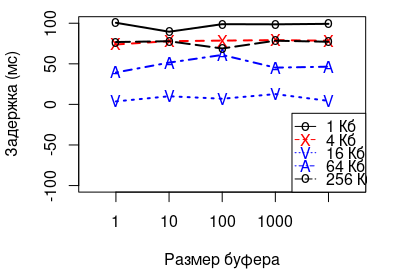
\includegraphics[width=\textwidth]{img/ros/ros_buf_l_k.png}
		\end{column}
		\begin{column}{0.45\textwidth}
			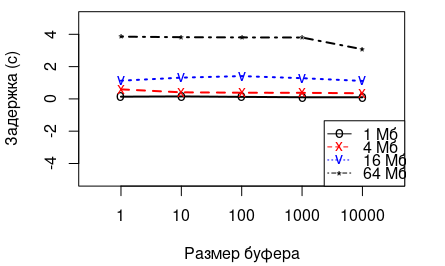
\includegraphics[width=\textwidth]{img/ros/ros_buf_l_m.png}
		\end{column}
	\end{columns}
	
	Количество подписчиков:
	\begin{columns}[onlytextwidth]
		\begin{column}{0.45\textwidth}
			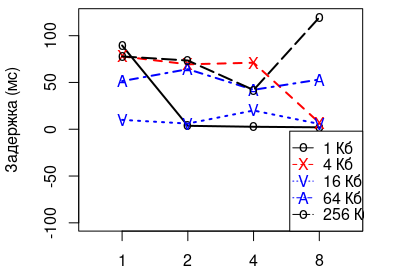
\includegraphics[width=\textwidth]{img/ros/ros_subs_l_k.png}
		\end{column}
		\begin{column}{0.45\textwidth}
			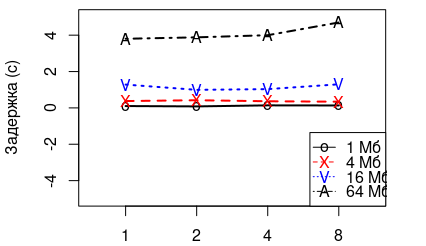
\includegraphics[width=\textwidth]{img/ros/ros_subs_l_m.png}
		\end{column}
	\end{columns}
\end{frame}

\begin{frame}{ROS - паттерн \enquote{Издатель-подписчик}}
	Задержка при передачи сообщений:
	\begin{center}
		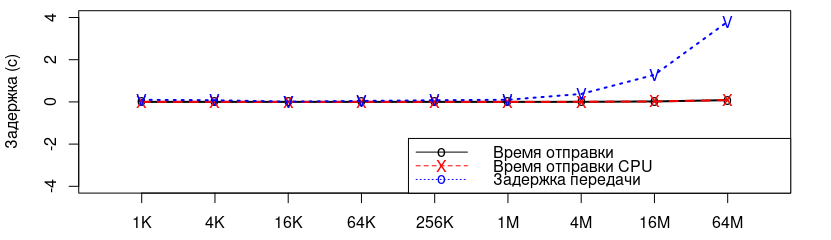
\includegraphics[width=.8\textwidth]{img/ros/ros_pubsub_l.png}
	\end{center}

	Пропускная способность:
	\begin{center}
		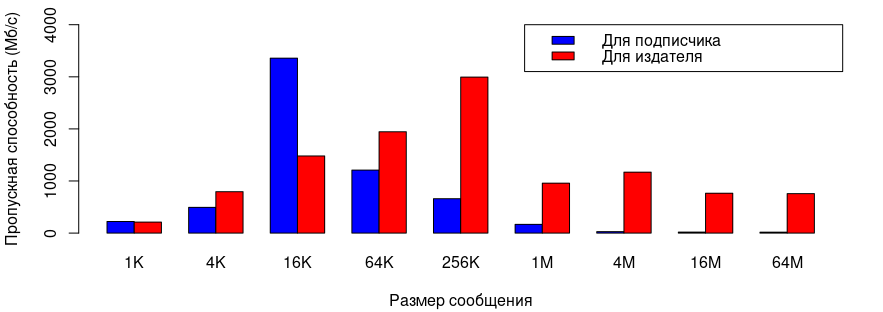
\includegraphics[width=.8\textwidth]{img/ros/ros_pubsub_bw.png}
	\end{center}
\end{frame}

\begin{frame}{ROS - паттерн \enquote{Клиент-сервис}}
Задержка передачи запроса и ответа:
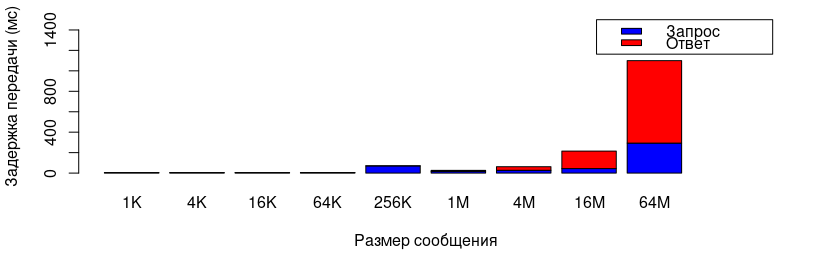
\includegraphics[width=\textwidth]{img/ros/ros_rpc_l.png}
Сравнение с подходом "издатель-подписчик":
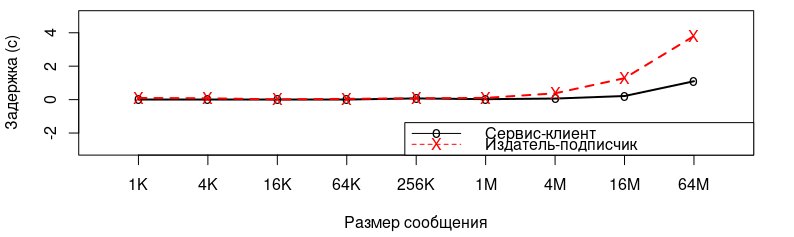
\includegraphics[width=\textwidth]{img/ros/ros_rpc_pubsub.png}
\end{frame}

\subsection{MIRA}
\begin{frame}{MIRA - зависимость от расположения модулей}
\begin{columns}[onlytextwidth]
	\begin{column}{0.45\textwidth}
		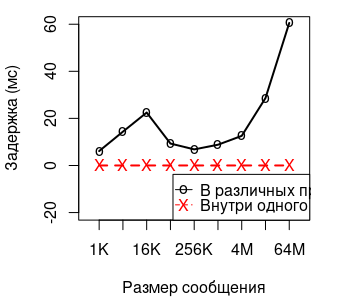
\includegraphics[width=\textwidth]{img/mira/mira_res_i_o_ml.png}
	\end{column}
	\begin{column}{0.45\textwidth}
		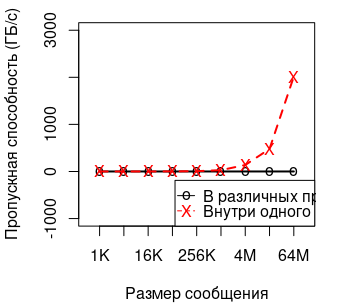
\includegraphics[width=\textwidth]{img/mira/mira_res_i_o_bps.png}
	\end{column}
\end{columns}
\end{frame}

\begin{frame}{MIRA - RPC}
	Сравнение задержки передачи данных с каналами:
	\begin{center}
		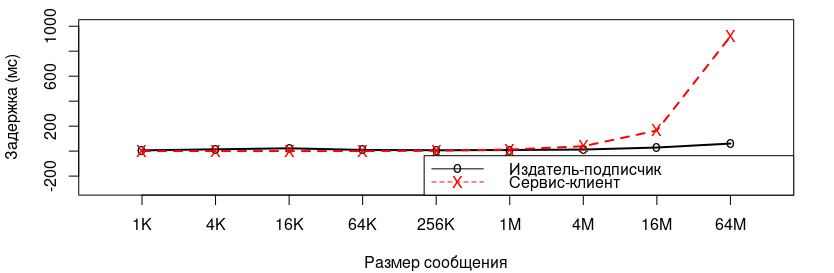
\includegraphics[width=.8\textwidth]{img/mira/mira_res_rpc_pubsub.png}
	\end{center}
	Пропускная способность:
	\begin{center}
		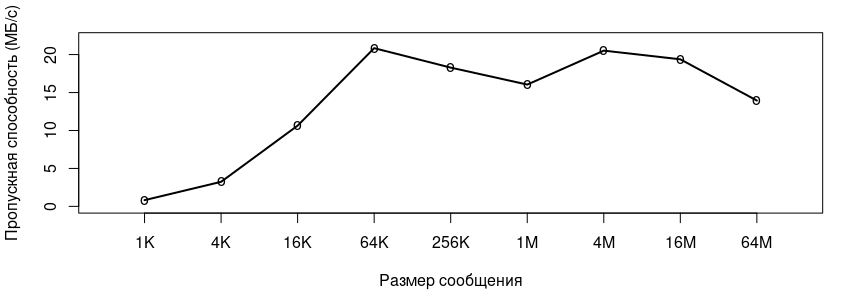
\includegraphics[width=.8\textwidth]{img/mira/mira_res_rpc_bps.png}
	\end{center}
\end{frame}

\subsection{YARP}
\begin{frame}{YARP - сравнение различных типов портов}
	Сравнение задержки передачи данных:
	\begin{center}
		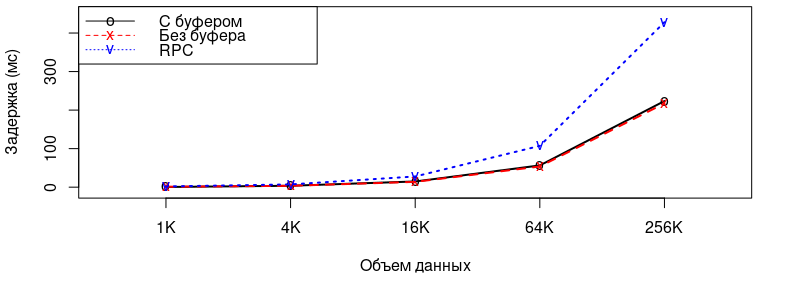
\includegraphics[width=.8\textwidth]{img/yarp/yarp_ports_l.png}
	\end{center}
	Сравнение пропускной способности:
	\begin{center}
		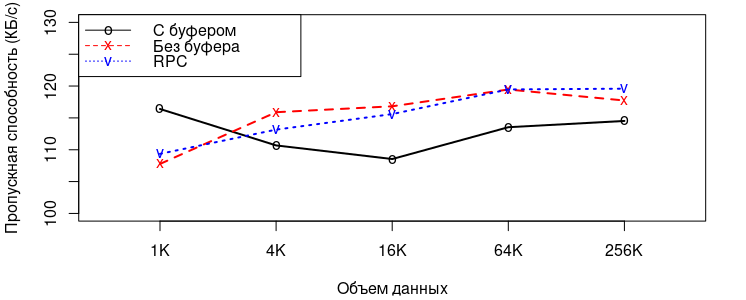
\includegraphics[width=.8\textwidth]{img/yarp/yarp_ports_bw.png}
	\end{center}
\end{frame}

\begin{frame}{YARP - сравнение различных протоколов}
Для буферизованного порта:
\begin{columns}[onlytextwidth]
	\begin{column}{0.5\textwidth}
		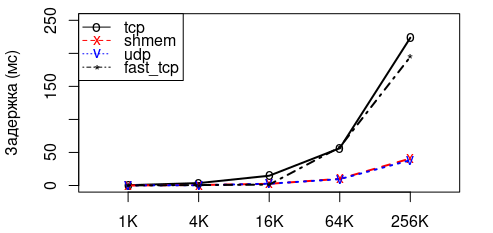
\includegraphics[width=\textwidth]{img/yarp/yarp_protocol_buf_l.png}
	\end{column}
	\begin{column}{0.5\textwidth}
		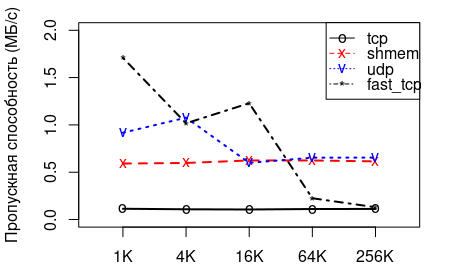
\includegraphics[width=\textwidth]{img/yarp/yarp_protocol_buf_bw.png}
	\end{column}
\end{columns}
Для RPC-порта:
\begin{columns}[onlytextwidth]
	\begin{column}{0.5\textwidth}
		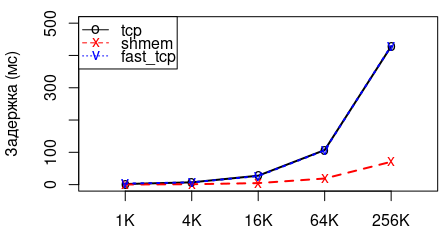
\includegraphics[width=\textwidth]{img/yarp/yarp_protocol_rpc_l.png}
	\end{column}
	\begin{column}{0.5\textwidth}
		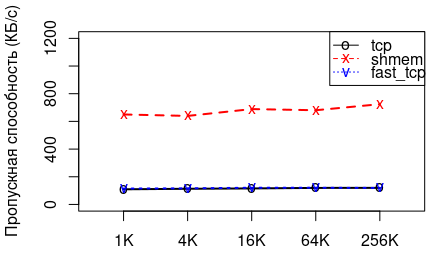
\includegraphics[width=\textwidth]{img/yarp/yarp_protocol_rpc_bw.png}
	\end{column}
\end{columns}
\end{frame}

\subsection{Сравнение}
\begin{frame}{Сравнение производительности фреймворков}
	Передача данных по TCP для различных процессов:
	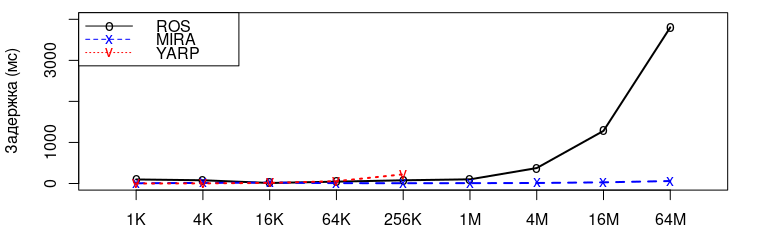
\includegraphics[width=\textwidth]{img/comp/comp_tcp_l.png}
	Производительность реализаций RPC:
	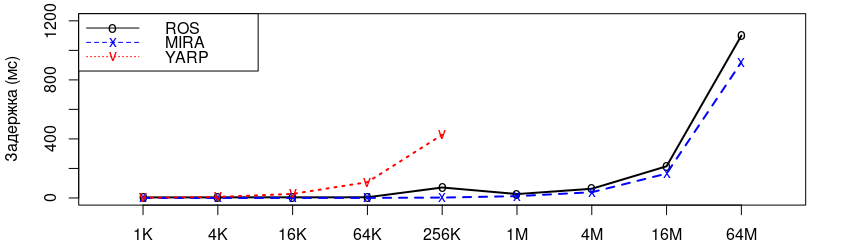
\includegraphics[width=\textwidth]{img/comp/comp_rpc_l.png}
\end{frame}

\subsection{Итоги}
\begin{frame}{Итоги тестирования производительности}
Таким образом, результаты тестирования выявили следующие факты:
\begin{itemize}
	\item на производительность ROS не влияет ни количество подписчиков, ни размер буфера
	\item производительность ROS резко падает при передачи больших объемов данных
	\item YARP имеет наихудшие показатели производительности
	\item в YARP рекомендуется использовать разделяемую память на основе ACE
	\item MIRA имеет наилучшие показатели производительности
\end{itemize}
\end{frame}
